\section{Сравнение методов глобальной оптимизации}

В предыдущем разделе был рассмотрен вопрос о выборе базовой схемы редукции размерности размерности задач оптимизации вида \ref{eq:task} для
алгоритма IAGS. В этом разделе рассмотрим сравнение алгоритма глобального поиска с одной развёрткой типа кривой Пеано
и других алгоритмов глобальной оптимизации, основанных на кардинально различных принципах. Такое сравнение позволит
выяснить, перспективен ли базовый алгоритм глобального поиска для дальнейших модификаций.
Как и ранее, в качестве тестовых задач для сравнения, будем рассматривать задачи без ограничений, поскольку большинство рассматриваемых методов
не предусматривают специально разработанных схем для их эффективного учёта.
Обозначим алгоритм глобального поиска без индексной схемы как AGS. Также рассмотрим схему контроля
параметра надёжности \(r\) в AGS, позволяющую в некоторых случаях снизить зависимость метода от его выбора.

\subsection{Методы глобальной оптимизации для сравнения}
\begin{itemize}
  \item \textbf{Multi Level Single Linkage} \cite{Kan1987StochasticGO}. MLSL является улучшенным вариантом мультистартовой схемы \cite{}.
  Алгоритм сэмплирует стартовые точки, равномерно распределённые по области посика, и производит локальную оптимизацию из них.
  В сравнении со стандартной мультистартовой схемой MLSL использует кластеризацию и набор эвристических правил
  для избежания повторных локальных спусков в уже обнаруженные лакальные минимумы.

  \item \textbf{DIRECT} \cite{Jones2009}. Метод является детерминированным и рекурсивно разделяет
  область поиска, формируя дерево гиперпрямоугольников. DIRECT использует значения целевой функции и
  оценку константы Липшица (\ref{eq:lip}) для получения оценки перспективности дальнейшего разбиения каждого из гиперинтервалов.

  \item \textbf{Locally-biased DIRECT (DIRECT$l$)} \cite{Gablonsky2001}. Вариация метода
  DIRECT, которая меньше уделяет внимания гиперинтервалам с низкой оценкой перспективности.
  Эта вариация сходится быстрее на задачах с небоьлшим количеством локальных минимумов,
  но в сложных случаях может не найти глобальный.

  \item \textbf{Dual Simulated Annealing} \cite{XIANG1997216}. Этот стохастический метода является комбинацией
  классическойго метода имитации отжига (CSA \cite{annealing}) и быстрого метода имитации отжига (FSA \cite{SZU1987157}), совмещенной
  с применением локальной оптимизации. Метод сходится гораздо быстрее, чем CSA и FSA.

  \item \textbf{Differential Evolution} \cite{Storn1997}. DE является адаптацией оригинального генетического алгоритма
  к непрерывному пространству поиска.

  \item \textbf{Controlled Random Search} \cite{Price1983}. CRS производит испытания в случайно сгенерированных начальных
  точках и определяет следующую точку для испытания на основе симплекса, построенного из случайно выбранных точек более ранних испытаний.
  CRS не считается эволюционным алгоритмом, хотя хранит точки, похожие на популяцию, и выполняет случайные трансформации над ними,
  по аналогии с применением оператора мутации.

  \item \textbf{StoGO} \cite{Madsen1998}. StoGO разделяет пространство поиска на гиперпрямогульники и использует метод ветвей и
  границ, вычисляя верхние оценки минимумов в подобластях с помощью локальной оптимизации.
\end{itemize}

Все перечисленные алгоритмы доступны в исходных кодах как компоненты широко распространённых программных пакетов.
DIRECT, DIRECT$l$, CRS, MLSL и StoGO являются компонентами библиотеки NLOpt \cite{nlopt}.
Реализации DE и DSA распространяются в пакете SciPy \cite{scipy} для языка Python.

\subsubsection{Контроль параметра надёжности в AGS}

Параметр $r$ из (\ref{eq:step2}) непосредственно влияет на глобальную сходимость AGS (см. \cite{Strongin2000}, Глава 8):
при достаточно большом значении $r$ метод гарантированно сходится ко всем глобальным минимумам целевой функции.
В то же время, согласно (\ref{eq:step3_1}), при бесконечно большом значении $r$ AGS превращается в полный перебор
по равномерной сетке.

В идеальном случае, для обеспечения наибольшей скорости сходимости оценка константы Липшица из (\ref{eq:step2})
не должна быть слишком завышенной, но на практике реальное значение $L$ из (\ref{eq:lip}) неизвестно и приходится
либо брать заведомо большое значение $r$, либо проводить несколько запусков AGS с разными параметрами. Чтобы в некотрой
степени решить обозначенную проблему выбора $r$ будем использовать следующую схему:
\begin{itemize}
  \item совершить $q$ итераций AGS при $r=r_{max}$;
  \item совершить $q$ итераций AGS при $r=r_{min}$;
  \item повторять предыдущие шаги до схоимости или исчерпания лимита итараций.
\end{itemize}

В указанном алгоритме $r_{min} < r_{max}$, $q > 1$. Вместо одного параметра $r$ теперь
необходимо выбирать 3, однако, согласно численным экспериментам, сделать это проще, чем найти оптимальное значение $r$.
Интуитивно практическую эффективность предложенной схемы можно объяснить тем, что теперь работа метода происходит в
двух режимах: глобальный поиск при $r=r_{max}$ и локальный при $r=r_{min}$. Если во время фазы глобального посика
метод приблизился к глобальному минимуму, то во время следующей фазы оценка глобального минимума будет быстро уточнена.
Если двух фаз не хватило, то процесс продолжается. Таким образом выбирается более оптимальный компромисс
между локальной и глобальной оптимизацией. Далее будем обозначать метод, использующий описанную схему как AGS-AR.

\subsection{Результаты численных экспериментов}
\label{sec:experiments}
Результаты решения методами задач глобальной оптимизации различной сложности напрямую зависят от
выбранных параметров методав. В большинстве случаев авторы программных реализаций ориентируются
на задачи средной сложности. Чтобы получить приемлемые результаты на существенно многоэкстремальных
задачах, параметры некоторых методов были выбраны слудующим образом:
\begin{itemize}
  \item в AGS-AR параметр чередования локальной и глобальной фаз $q$ был выбран равным $50\cdot\log_2(N-1)\cdot N^2$, а $r_{min}=3,\:r_{max}=2\cdot r_{min}$;
  \item в DIRECT и DIRECT\(l\) параметр \(\epsilon=10^{-4}\);
  \item в SDA параметр \(visit=2.72\).
\end{itemize}

Остальные параметры варьировались в зависимости от набора тестовых задач (см. Таблицу~\ref{tab:params}).
Для AGS минимальное значение параметра $r$ такое, что все задачи заданного класса решаются, было получено перебором по равномерной сетке с шагом $0.1$.

\begin{table}
\begin{center}
\caption{Параметры методов оптимизации для различных тестовых задач}
  \begin{tabular}{|l|{c}|{c}|{c}|}
    \hline
    & AGS & CRS & DE\\
  \hline
  \(F_{GR}\) & \(r=3\) & popsize=150 & mutation=(1.1,1.9), popsize=60 \\
  \hline
  GKLS 2d Simple & \(r=4.6\) & popsize=200 & mutation=(1.1,1.9), popsize=60 \\
  \hline
  GKLS 2d Hard & \(r=6.5\) & popsize=400 & mutation=(1.1,1.9), popsize=60 \\
  \hline
  GKLS 3d Simple & \(r=3.7\) & popsize=1000 & mutation=(1.1,1.9), popsize=70 \\
  \hline
  GKLS 3d Hard & \(r=4.4\) & popsize=2000 & mutation=(1.1,1.9), popsize=80 \\
  \hline
  GKLS 4d Simple & \(r=4.7\) & popsize=8000 & mutation=(1.1,1.9), popsize=90 \\
  \hline
  GKLS 4d Hard & \(r=4.9\) & popsize=16000 & mutation=(1.1,1.9), popsize=100 \\
  \hline
  GKLS 5d Simple & \(r=4\) & popsize=25000 & mutation=(1.1,1.9), popsize=120 \\
  \hline
  GKLS 5d Hard & \(r=4\) & popsize=30000 & mutation=(1.1,1.9), popsize=140 \\
  \hline
\end{tabular}
  \label{tab:params}
\end{center}
\end{table}

\begin{table}
\begin{center}
\caption{Среднее количество испытаний, затраченное методами оптимизации при решении задач различных классов}
\resizebox{\textwidth}{!}{%
  \begin{tabular}{|l|{c}|{c}|{c}|{c}|{c}|{c}|{c}|{c}|{c}|{c}|}
    \hline
    & AGS & AGS-AR & CRS & DIRECT & DIRECT\(l\) & MLSL & SDA & DE & StoGO \\
  \hline
  \(F_{GR}\)     & 193.1 & 248.3 & 400.3 & \textbf{182.2} & 214.9 & 947.2 & 691.2 & 1257.3 & 1336.8 \\
  \hline
  GKLS 2d Simple & 254.9 & 221.6 & 510.6 & \textbf{189.0} & 255.2 & 556.8 & 356.3 & 952.2 & 1251.5 \\
  \hline
  GKLS 2d Hard   & \textbf{728.7} & 785.0 & 844.7 & 985.4 & 1126.7 & 1042.5 & 1637.9 & 1041.1 & 2532.2 \\
  \hline
  GKLS 3d Simple &  1372.1 & 1169.5 & 4145.8 & \textbf{973.6} & 1477.8 & 4609.2 & 2706.5 & 5956.9 & 3856.1 \\
  \hline
  GKLS 3d Hard   &  3636.1 & \textbf{1952.1} & 6787.0 & 2298.7 & 3553.3 & 5640.1 & 4708.4 & 6914.3 & 7843.2 \\
  \hline
  GKLS 4d Simple &  5729.8 & \textbf{4919.1} & 19883.6 & 7328.8 & 15010.0 & 41484.8 & 22066.0 & 6271.2 & 29359.2 \\
  \hline
  GKLS 4d Hard   &  13113.4 & \textbf{12860.1} & 27137.4 & 22884.4 & 55596.1 & 80220.1 & 68048.0 & 12487.6 & 58925.5  \\
  \hline
  GKLS 5d Simple &  \textbf{5821.5} & 6241.3 & 62921.7 & 5966.1 & 10795.5 & 52609.2 & 34208.8 & 20859.4 & 69206.8 \\
  \hline
  GKLS 5d Hard   &  \textbf{17008.6} & 21555.1 & 87563.9 & 61657.3 & 148637.8 & 138011.8 & 115634.6 & 26850.0 & 141886.5 \\
  \hline
\end{tabular}}
  \label{tab:trials}
\end{center}
\end{table}

Результаты запуска рассматриваемых методов оптимизации на наборах тестовых задач представлены в таблицах \ref{tab:trials}, \ref{tab:solved}.
DIRECT, AGS, AGS-AR продемонстрировали лучшую скорость сходимости на всех классах, при этом AGS-AR уступает DIRECT
на двухмерных задачах класса Simple, но имеет преимущество на задачах класса Hard. Как можно видеть из Table~\ref{tab:solved},
детерминированные методы (AGS, AGS-AR, DIRECT и DIRECT\(l\)) оказались более надёжными, т.е. решили больше тестовых задач.
Среди стохастических методов самую высокую надёжность показали MLSL и SDA.

\begin{table}
\begin{center}
\caption{Количество задач оптимизации, решённых методами при заданном лимите испытаний (общее количество задач в каждом наборе равно 100)}
  \begin{tabular}{|l|{c}|{c}|{c}|{c}|{c}|{c}|{c}|{c}|{c}|{c}|}
    \hline
    & AGS & AGS-AR & CRS & DIRECT & DIRECT\(l\) & MLSL & SDA & DE & StoGO \\
  \hline
  \(F_{GR}\)     &  100 & 100 & 76 & 100 & 100 & 97 & 96 & 96 & 67\\
  \hline
  GKLS 2d Simple &  100 & 100 & 85 & 100 & 100 & 100 & 100 & 98 & 90\\
  \hline
  GKLS 2d Hard   &  100 & 97 & 74 & 100 & 100 & 100 & 93 & 85 & 77 \\
  \hline
  GKLS 3d Simple &  100 & 100 & 75 & 100 & 100 & 100 & 89 & 86 & 44 \\
  \hline
  GKLS 3d Hard   &  100 & 100 & 72 & 100 & 99 & 100 & 88 & 77 & 43 \\
  \hline
  GKLS 4d Simple &  100 & 100 & 74 & 100 & 100 & 94 & 82 & 68 & 72 \\
  \hline
  GKLS 4d Hard   &  100 & 100 & 60 & 99 & 99 & 94 & 73 & 55 & 69  \\
  \hline
  GKLS 5d Simple &  100 & 100 & 86 & 100 & 100 & 98 & 100 & 88 & 82  \\
  \hline
  GKLS 5d Hard   &  100 & 100 & 77 & 100 & 93 & 79 & 86 & 77 & 78 \\
  \hline
  \end{tabular}
  \label{tab:solved}
\end{center}
\end{table}

\begin{figure}[ht]
  \centering
  \subfloat[4d Simple]{{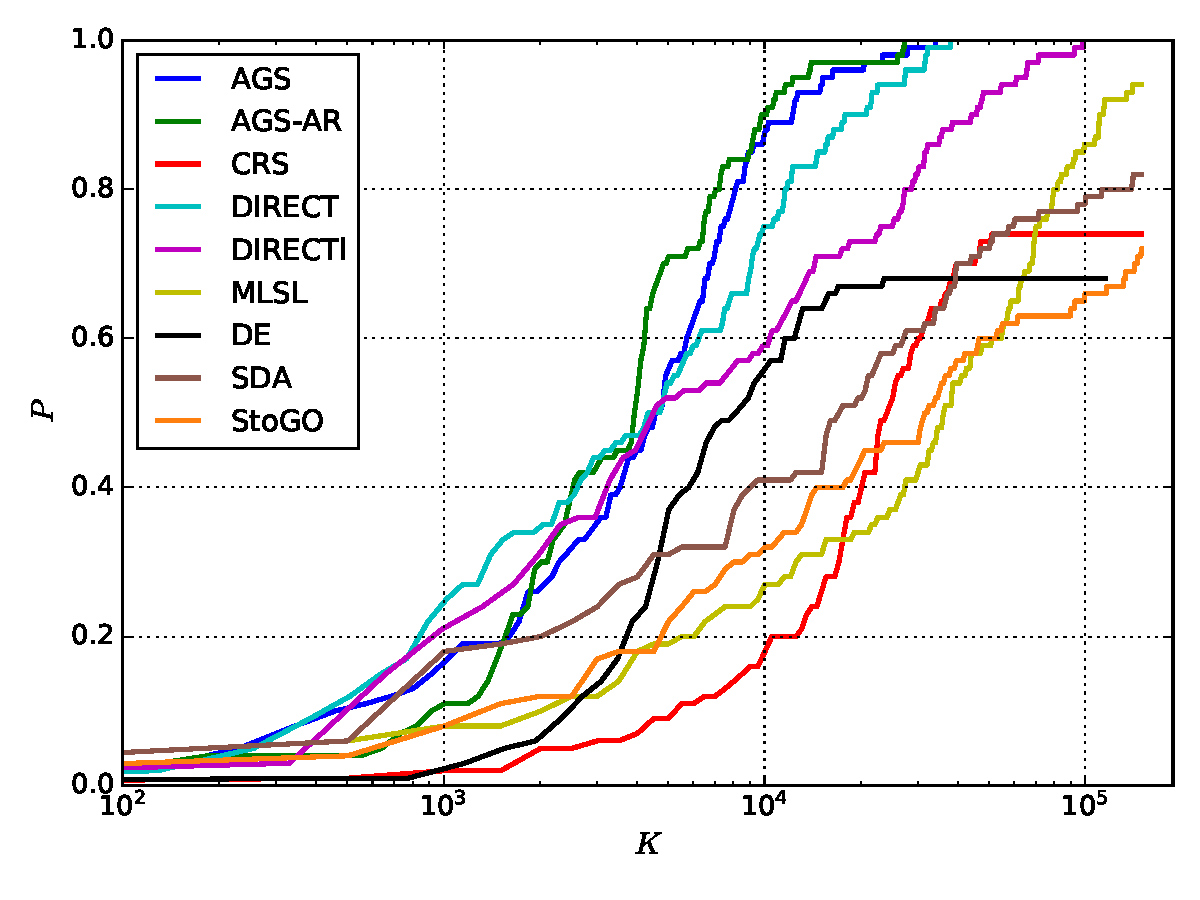
\includegraphics[width=.5\textwidth]{comparison/gklss4d.pdf}}\label{fig:s4d}}
  \subfloat[4d Hard]{{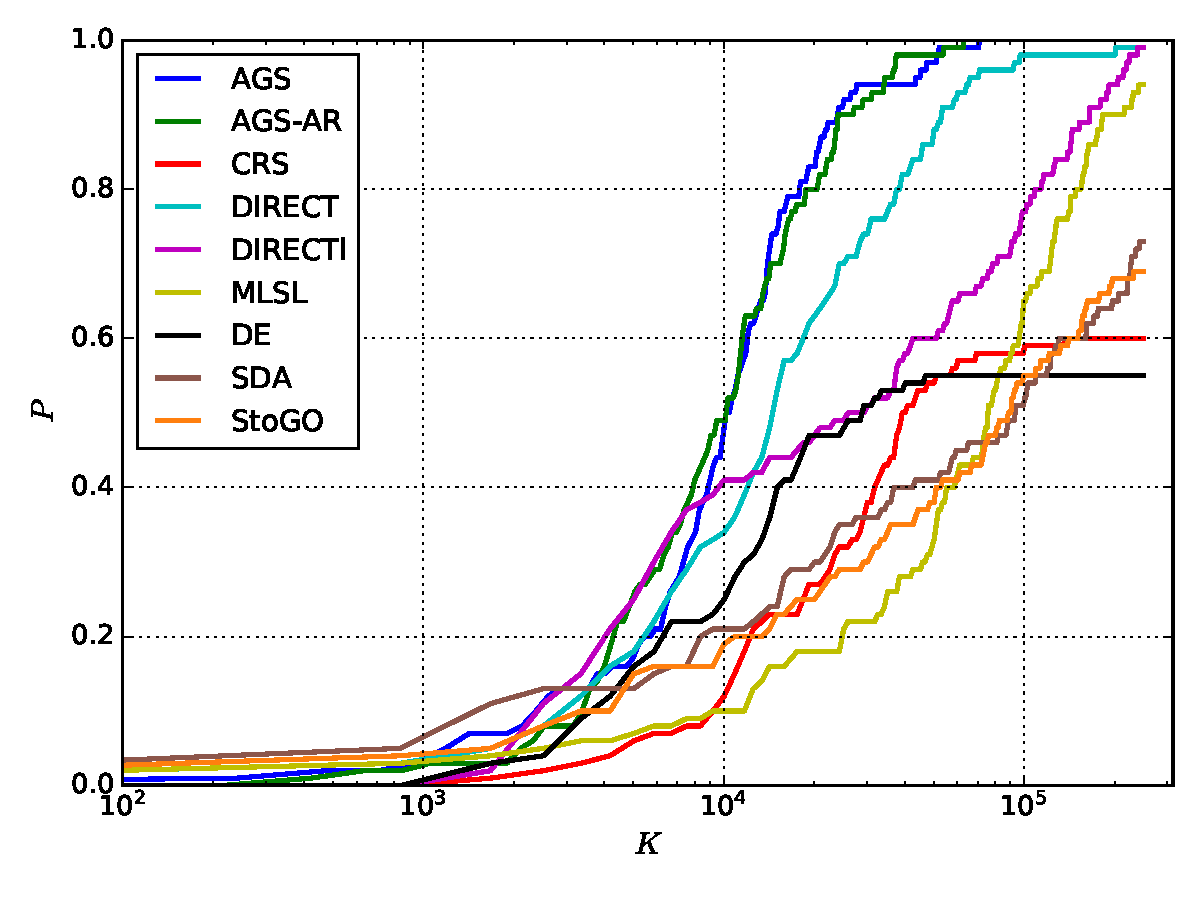
\includegraphics[width=.5\textwidth]{comparison/gklsh4d.pdf}}\label{fig:h4d}}

  \subfloat[5d Simple]{{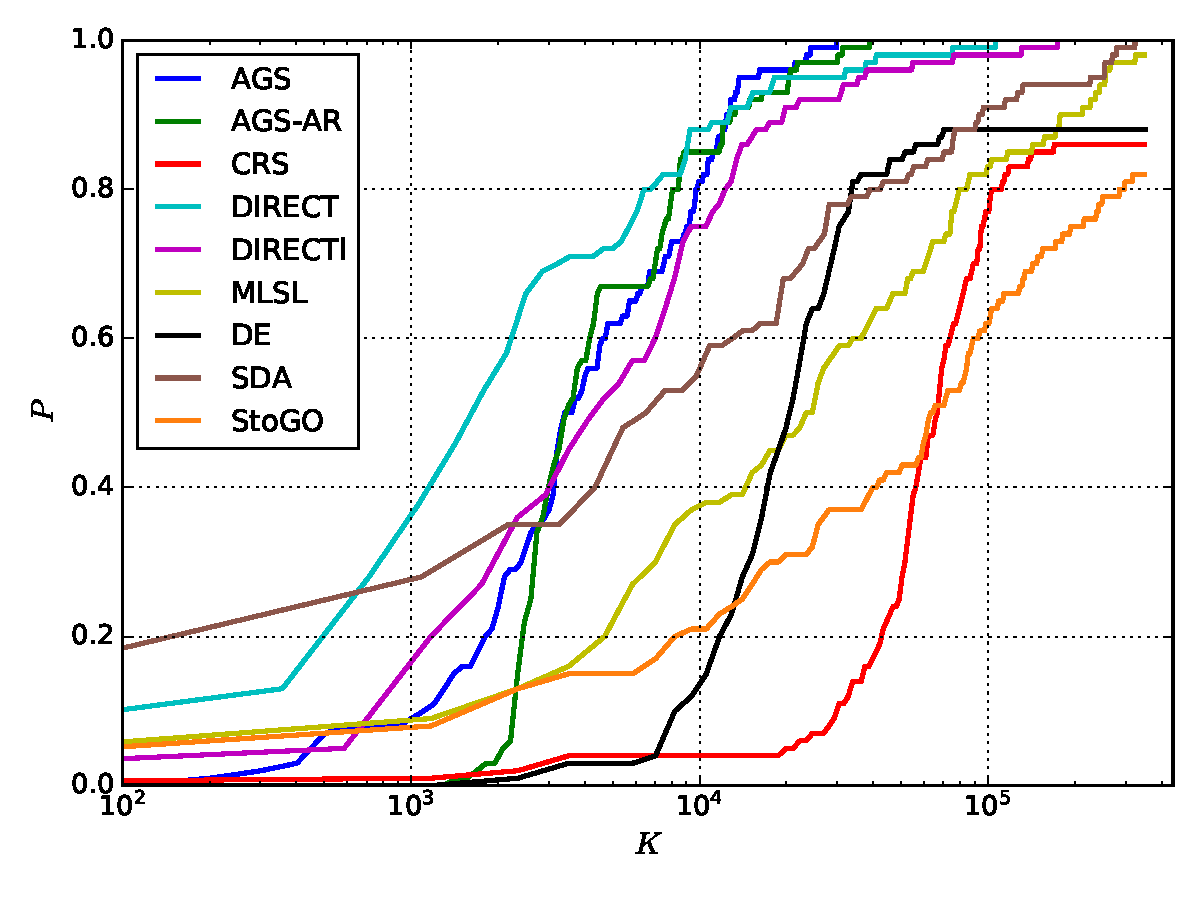
\includegraphics[width=.5\textwidth]{comparison/gklss5d.pdf}}\label{fig:s5d}}
  \subfloat[5d Hard]{{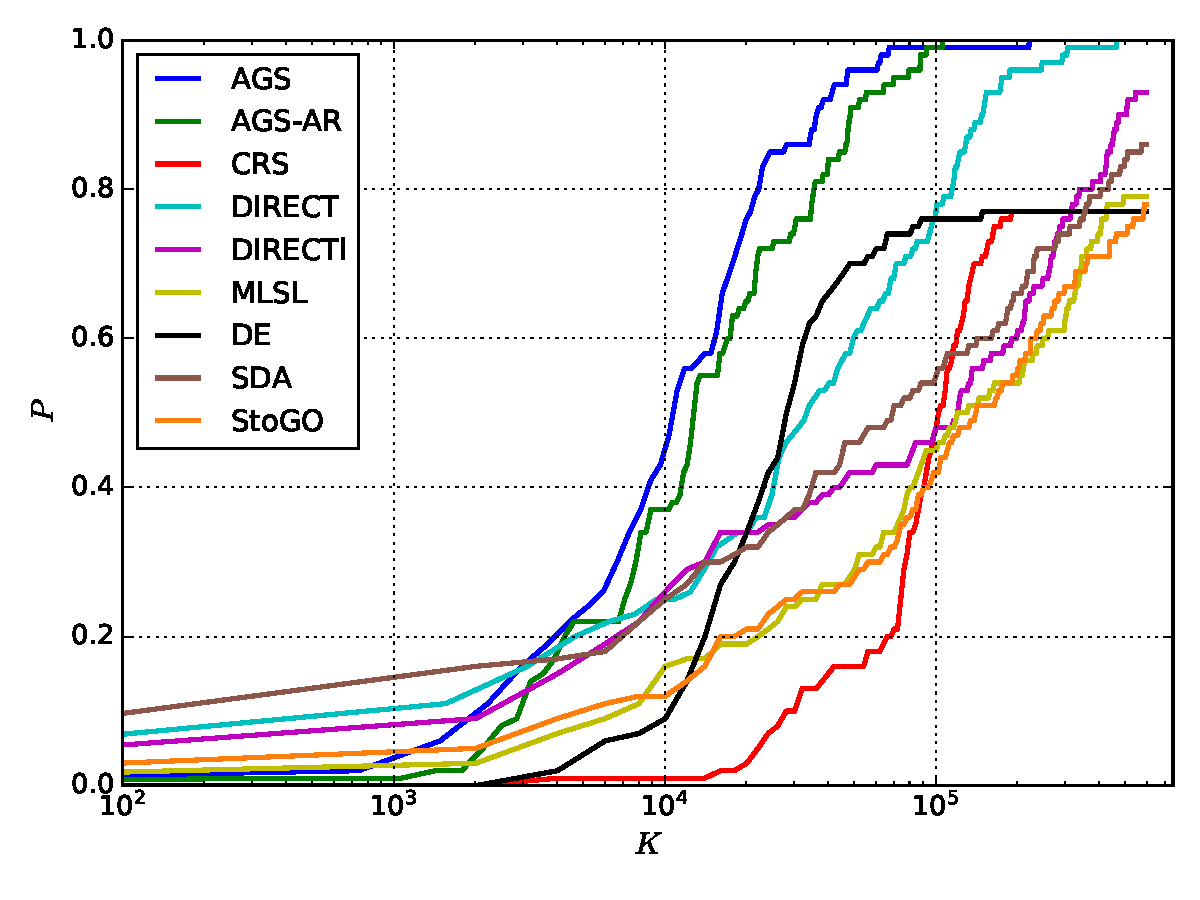
\includegraphics[width=.5\textwidth]{comparison/gklsh5d.pdf}}\label{fig:h5d}}
  \caption{Операционные характеристики методов при решении задач из классов GKLS 4d и 5d.}
\end{figure}

Операционные характеристики методов (Рис. \ref{fig:s4d}, \ref{fig:h4d}, \ref{fig:s5d}, \ref{fig:h5d})
показывают, что AGS и AGS-AR быстрее других методов достигают 100\% надёжности. Также на классе GKLS 5d Simple DIRECT
имеет скорость сходимости выше, чем у других методов, но есть несколько сложных задач, решение которые решаются существенно дольше других,
что влияет на среднее количество испытаний.

\paragraph{Чувствительность AGS и AGS-AR к выбору параметров.}

Чтобы оценить степень влияния настроек методов на скорость сходимости AGS и AGS-AR, были проведены
эксперименты на классе задач GKLS 5d Simple со следующими параметрами:
\begin{itemize}
  \item AGS при $r=4$ (как в Таблице~\ref{tab:params});
  \item AGS при $r=6$;
  \item AGS-AR с параметрами, указанными в начале Секции~\ref{sec:experiments}
  ($q=50\cdot\log_2(4)\cdot 25 = 2500$, $r_{min}=3,\:r_{max}=2\cdot r_{min}$);
  \item AGS-AR при $r_{max}=8$ and и остальными параметрами как в предыдущем эксперименте;
  \item AGS-AR при $q=1000$ и другими параметрами как в начале Секции~\ref{sec:experiments}.
\end{itemize}

\begin{figure}[ht]
  \centering
  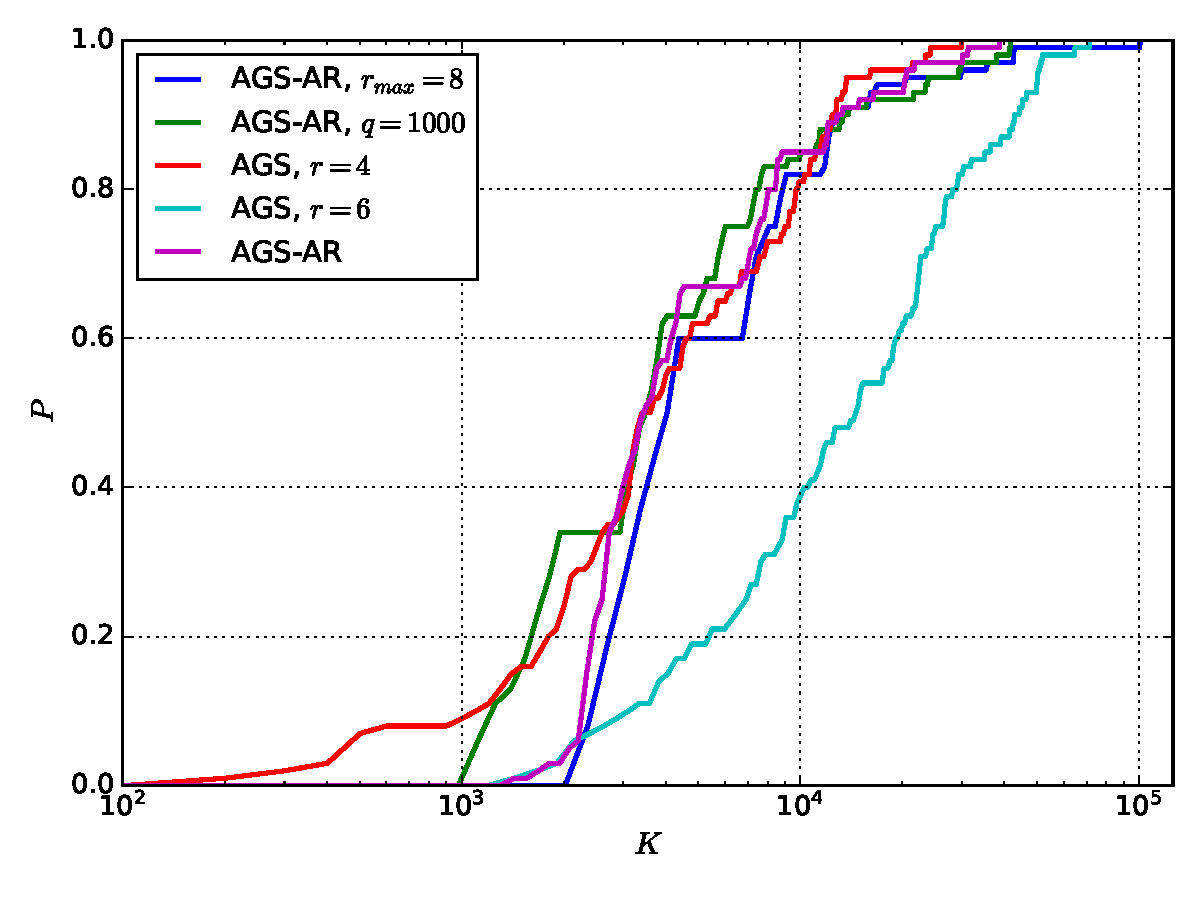
\includegraphics[width=.6\textwidth]{comparison/ar_stab.pdf}
  \caption{Операционные характеристики AGS и AGS-AR на классе GKLS 5d Simple
  с различными параметрами.}
  \label{fig:stability}
\end{figure}

Операционные характеристики, полученные в экспериментах, описанных выше, представлены на Рис.~\ref{fig:stability}.
AGS при $r=6$ (голубая кривая) показывает самую медленную сходимость, что говорит о высокой чувствительности AGS
к выбору значения $r$. Поскольку AGS-AR используе то же самое значение $r$ как AGS при $r=6$, операционные характеристики
этих методов идентичны до точки $K=2500$. После этой границы AGS-AR переключается на $r=3$ и количество решённых задач
начинает быстро возрастать, вплоть до начала следующей фазы глобального поиска при $K=5000$. Интервалы, на которых
AGS-AR работает с $r=r_{max}$ видны на операционных характеристиках как плато. Изменение $r$ и $q$ влияет на операционнух характеристику
AGS-AR незнаичтельно. Это наблюдение подтверждает надёжность предложенной модификации AGS с переменным параметром $r$.

\subsection{Итоги сравнения методов}

В результате сравнения разлиыных методов оптимизации, были сделаны следующие выводы:
\begin{itemize}
  \item предложенная модификация AGS, AGS-AR менее чувствительна к параметрам и сходится так же быстро, как AGS
  с заранее подобранными под класс задач параметрами;
  \item AGS-AR продемонстрировал надёжность и скорость сходимости на уровне удргого детеримнированного метода, DIRECT,
  и превзошёл на рассмотрнных тестовых задачах многие другие методы, реализации которых так же доступны в исходных кодах;
  \item на рассмотренных существенно многоэкстремальных задачах малой размерности стохастические методы оптимизации
  существенно уступают в скорости сходимости и надёжности детерминированным.
\end{itemize}
